\chapter{User Interface}

The application starts with the login page where the client is prompted to log-in or register into the application. 

\begin{figure}[H]
    \centering
    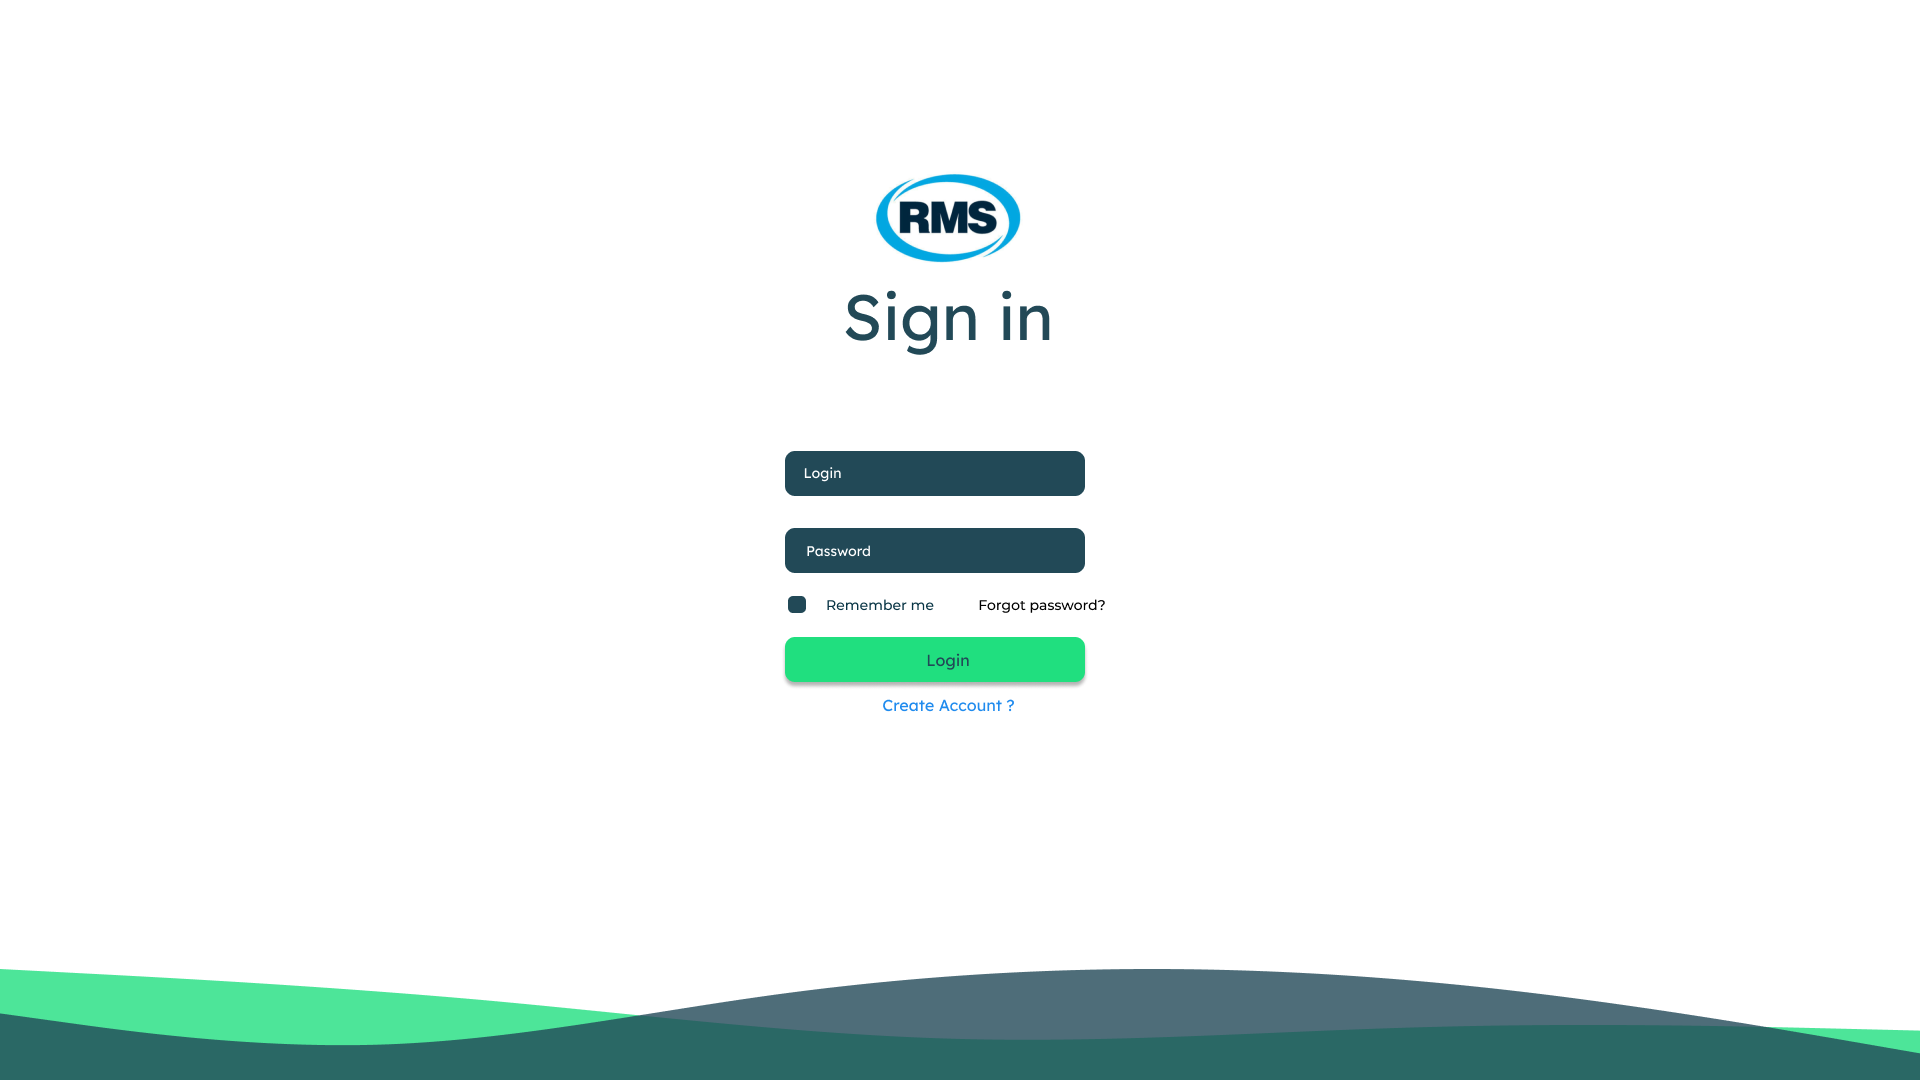
\includegraphics[scale=0.2]{images/Login Page.png}
    \caption{Sign-In Page}
    \label{fig:login-page}
\end{figure}
Once a super admin has logged in, they will see a grid of all the facilities available in the institute.
\begin{figure}[H]
    \centering
    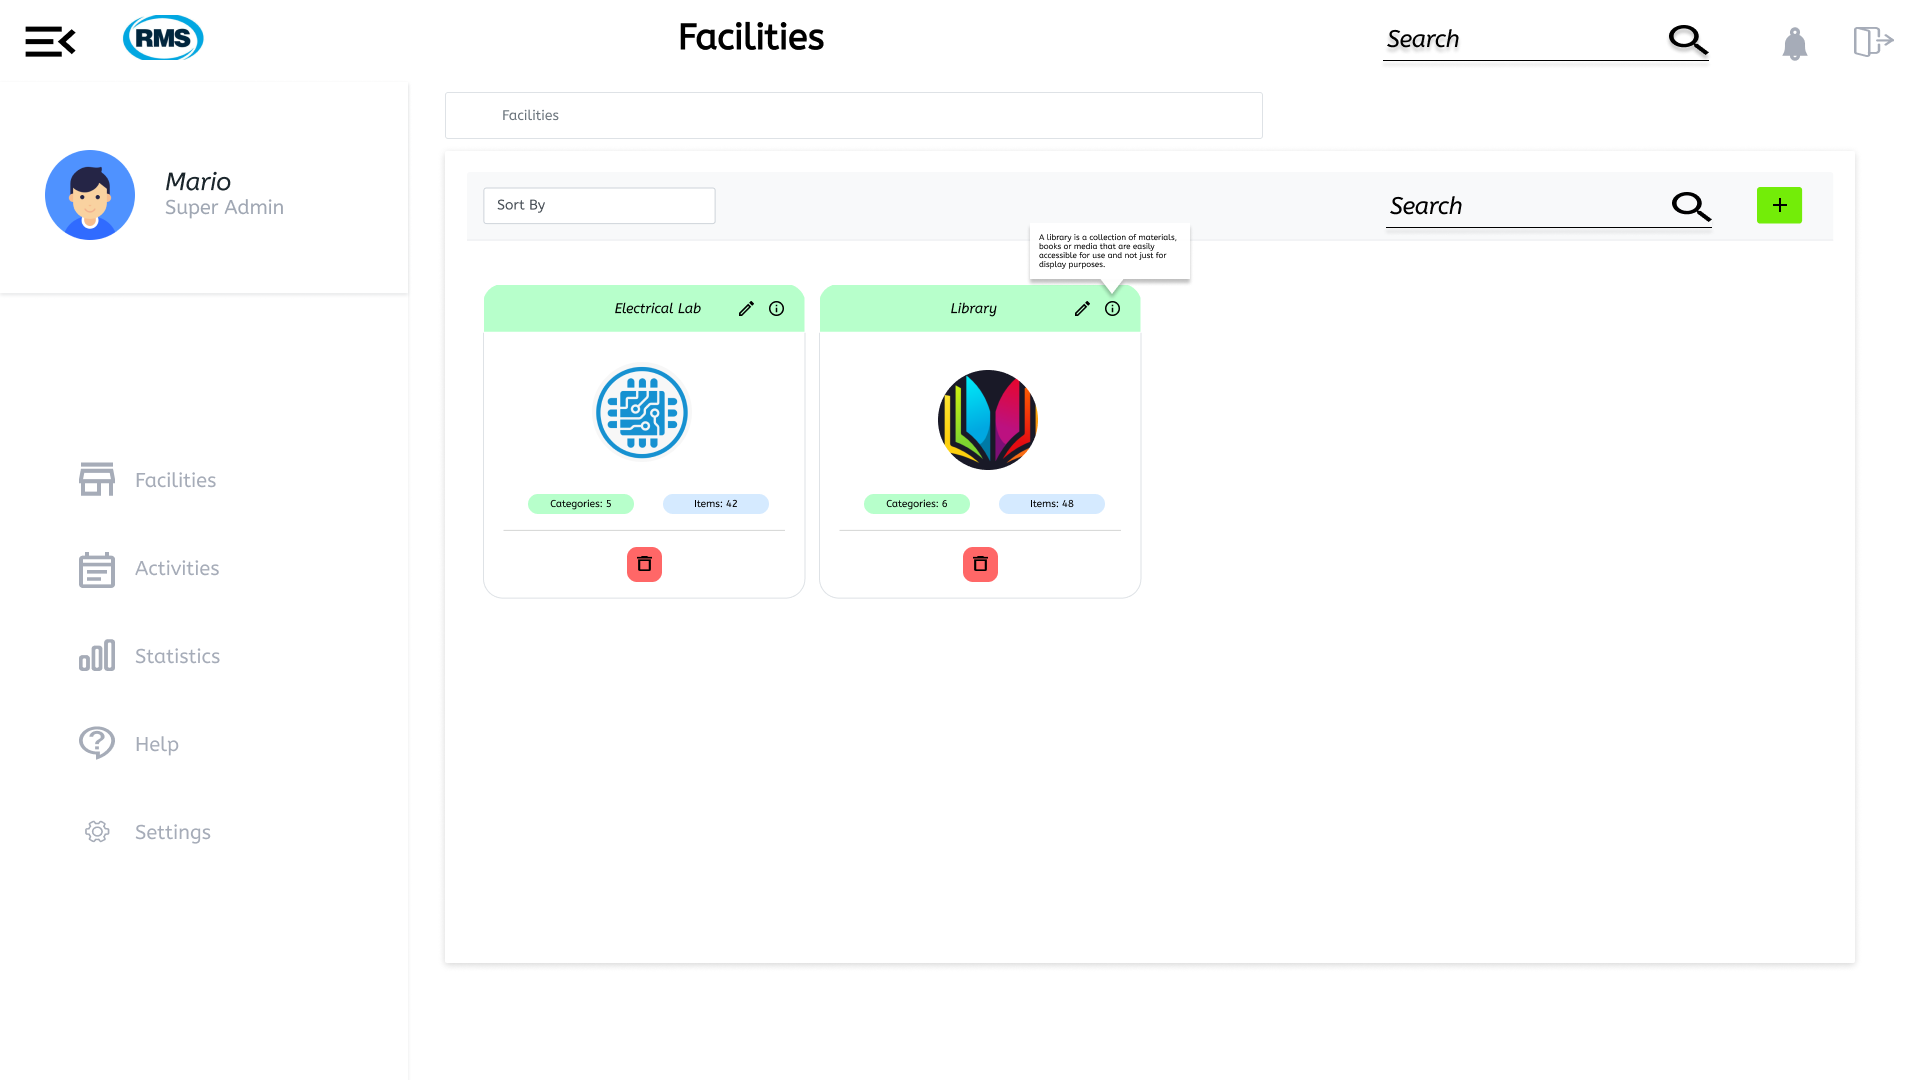
\includegraphics[scale=0.2]{images/Facilities.png}
    \caption{All facilities page}
    \label{fig:facilities}
\end{figure}
Every facility has an info button, upon being hovered shows a brief description of the facility. (As shown in Library) 
When the user clicks on a facility, they will see all the categories or items in that facility. Clicking on a category recursively shows all the categories or items in it, similar to the image below. 
\begin{figure}[H]
    \centering
    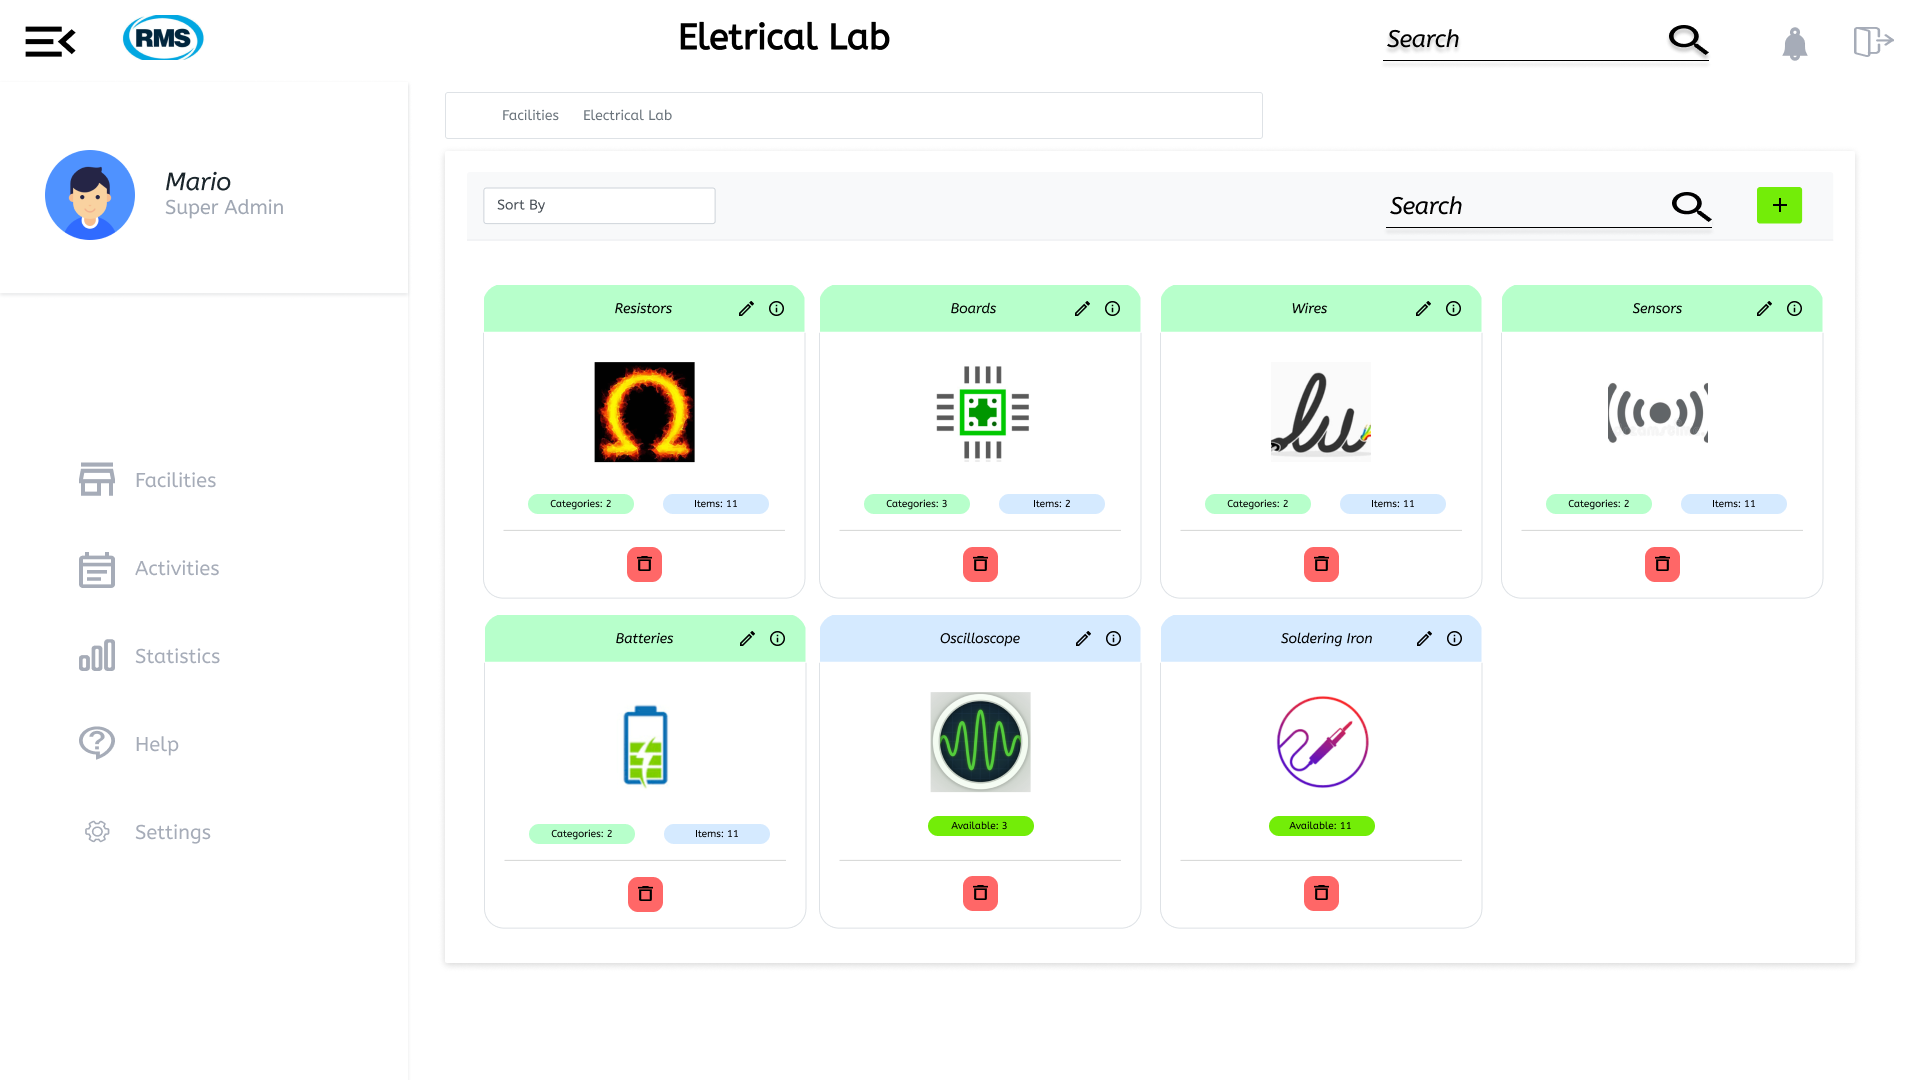
\includegraphics[scale=0.2]{images/Facility Info.png}
    \caption{Facility page}
    \label{fig:facility}
\end{figure}
To add a new category the user can click on the plus button in the top right of the grid. Upon clicking a dialog box as shown below pops up. 
\begin{figure}[H]
    \centering
    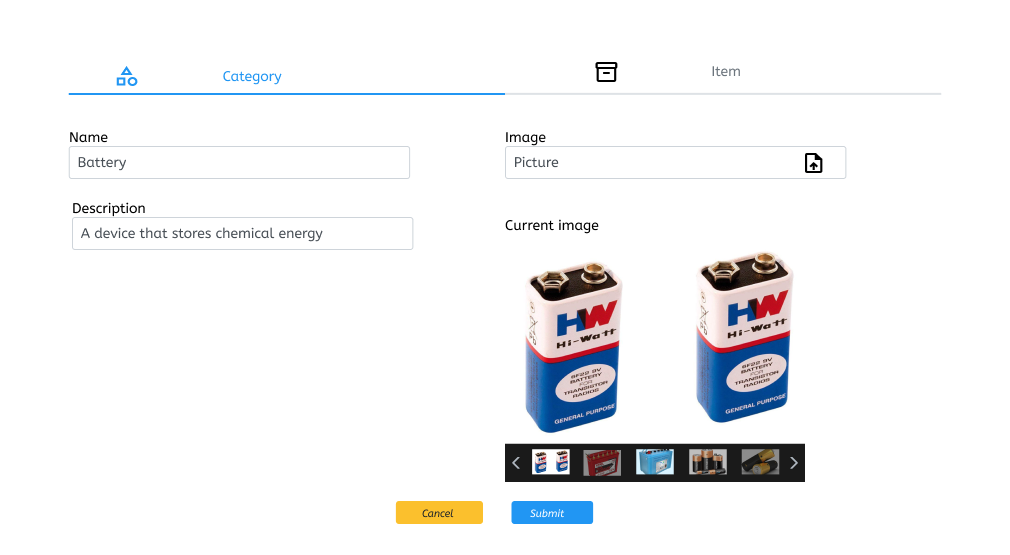
\includegraphics[scale=0.32]{images/CreateUpdate Category.png}
    \caption{Create or update category details.}
    \label{fig:cu-category}
\end{figure}
The user can fill in the fields with appropriate values and can create a category upon clicking the submit button.
Similarly the user can add new item by switching the tab in the pop-up as shown below.
\begin{figure}[H]
    \centering
    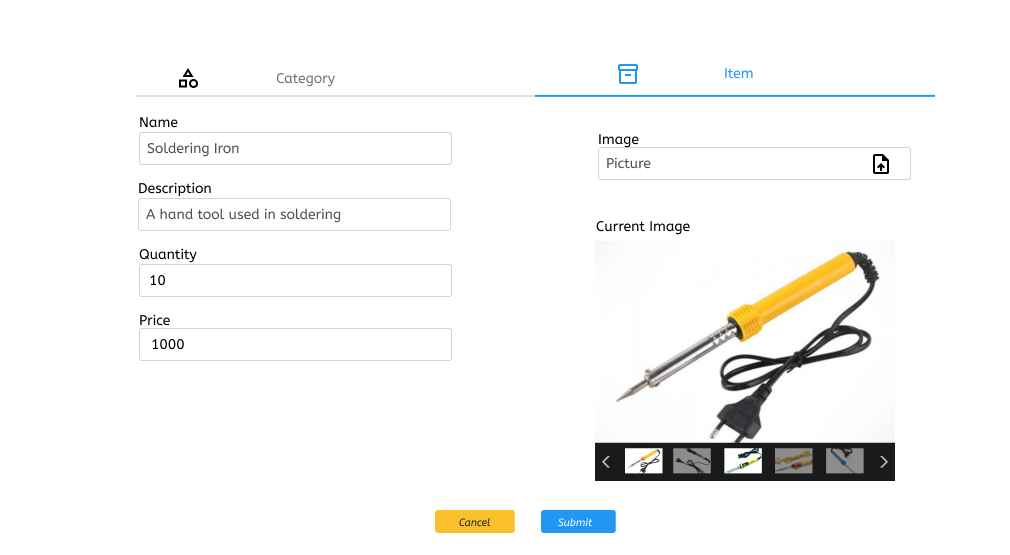
\includegraphics[scale=0.32]{images/CreateUpdate Item.png}
    \caption{Create or update item details.}
    \label{fig:cu-item}
\end{figure}
The user can fill in the fields with appropriate values and can create an item upon clicking the submit button. 
\clearpage
When the user clicks on an item in the grid, they will be directed to the item’s page as shown below. 
\begin{figure}[H]
    \centering
    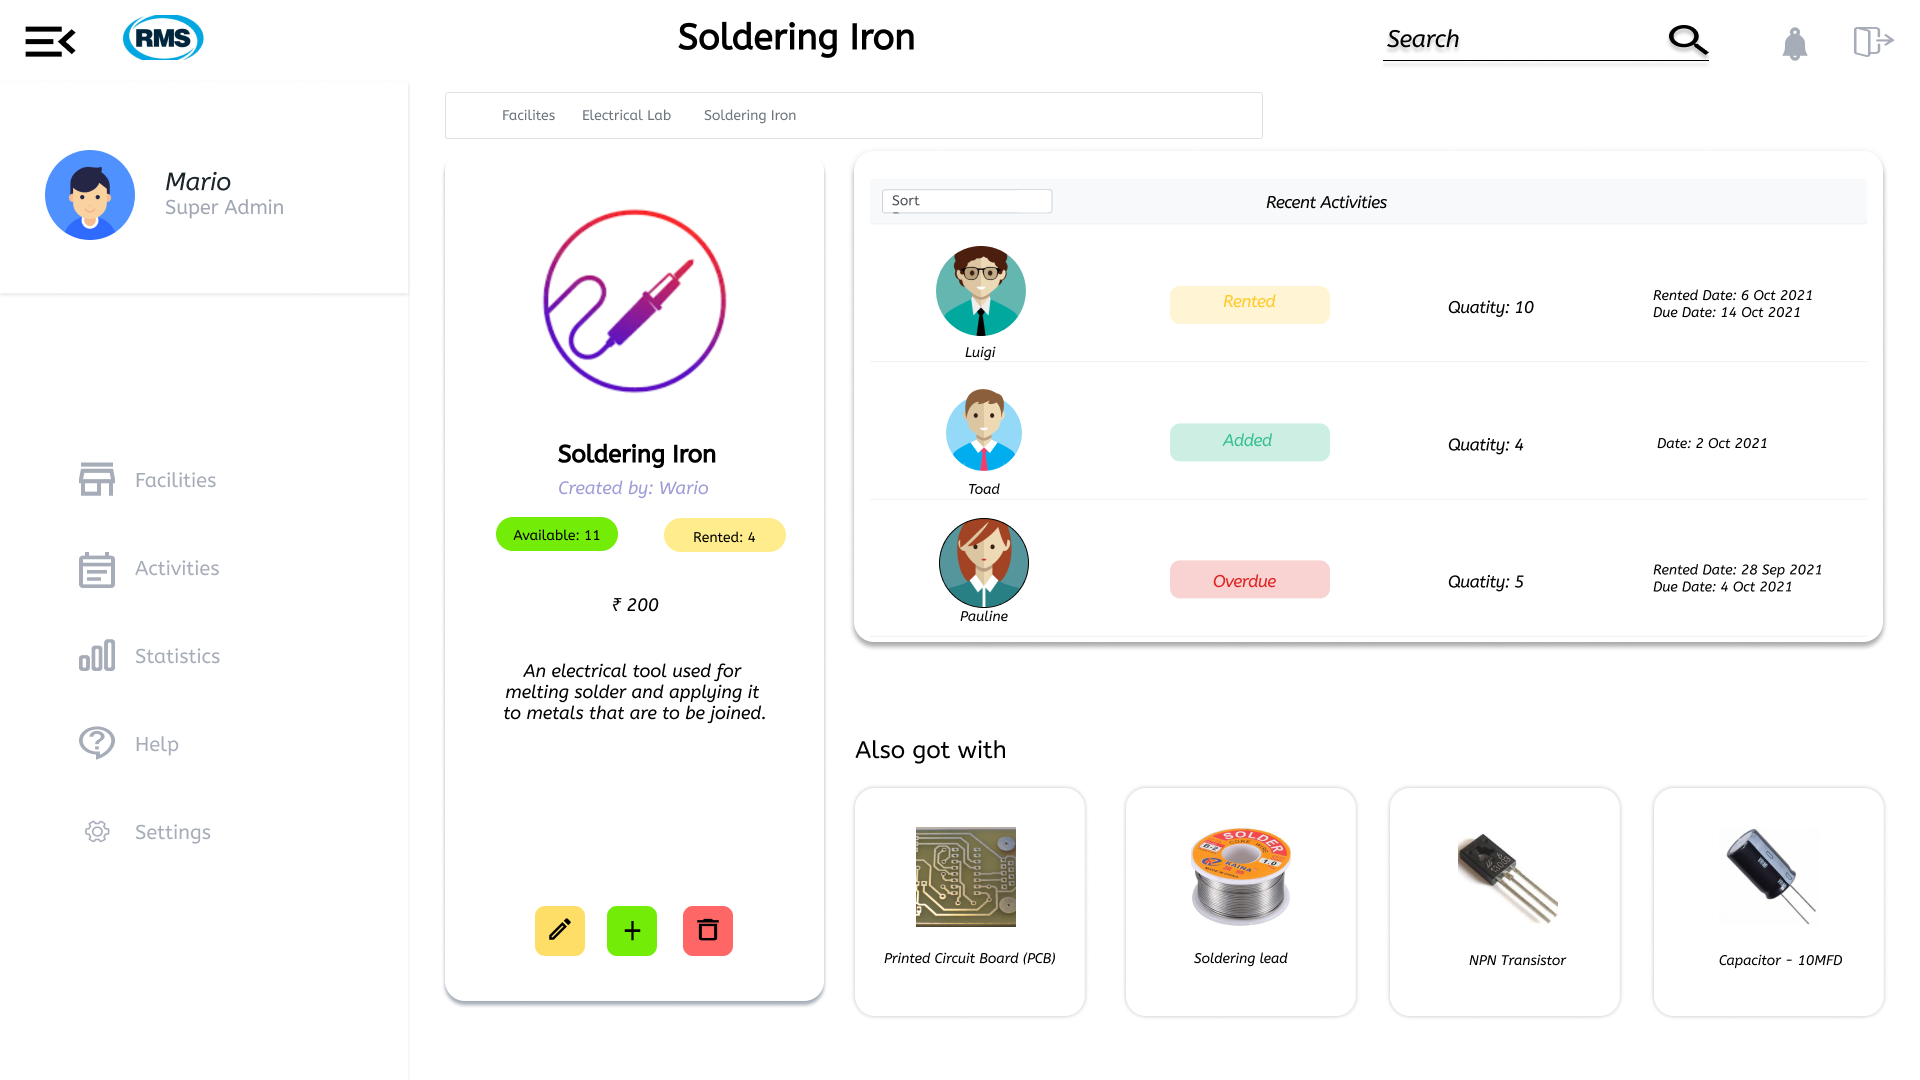
\includegraphics[scale=0.2]{images/Item Page.png}
    \caption{Detailed view of an item.}
    \label{fig:item}
\end{figure}
The item page has three panels: the item display, recent activities, and “Also got with” panel. The item display shows the created user, average cost, the description and some necessary action buttons. The recent activities show the list of user activates on this item. The “Also got with” panel shows the items that were most frequently brought with this item.
\clearpage
The admin can see all the activities that happen in the institute as shown below. 
\begin{figure}[H]
    \centering
    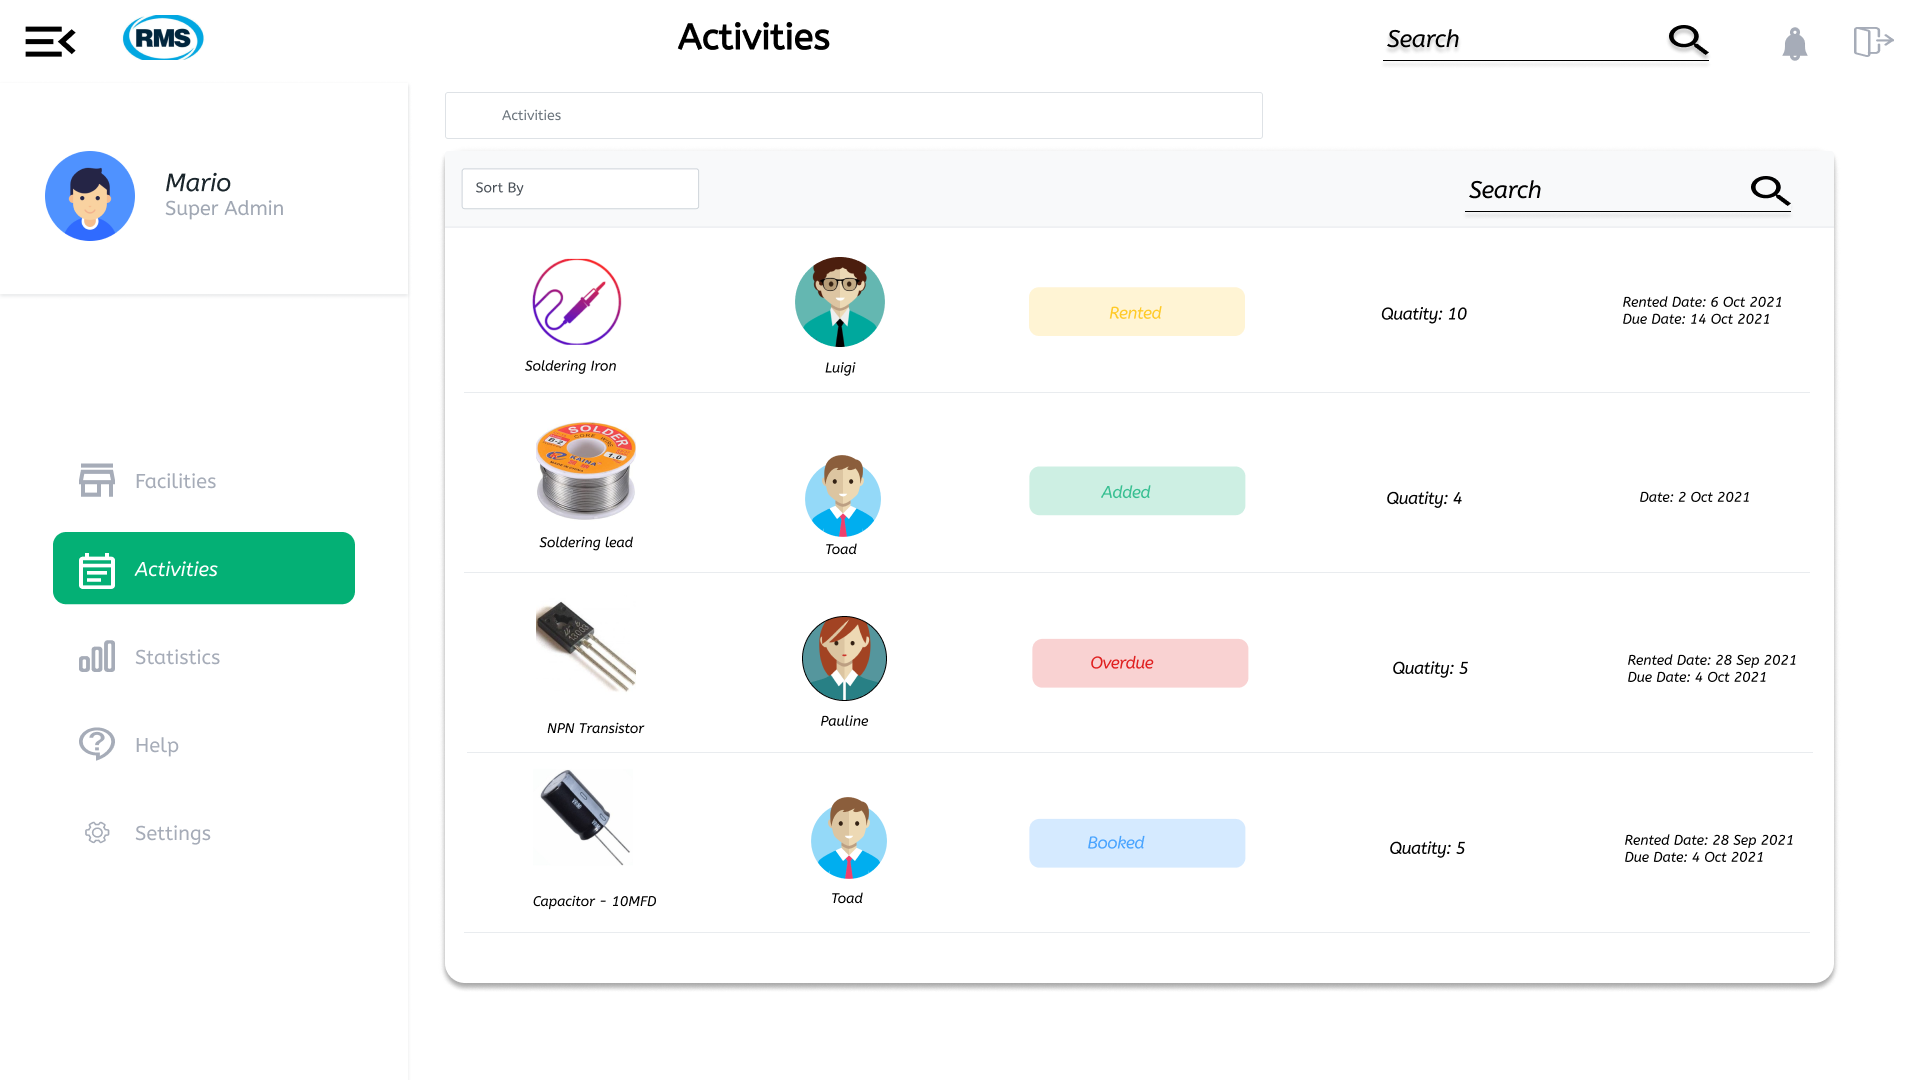
\includegraphics[scale=0.2]{images/Activities.png}
    \caption{All recent activities.}
    \label{fig:activities}
\end{figure}